\documentclass[a4paper]{article}

%% Language and font encodings
\usepackage[english]{babel}
\usepackage[utf8x]{inputenc}
\usepackage[T1]{fontenc}

%% Sets page size and margins
\usepackage[a4paper,top=3cm,bottom=2cm,left=3cm,right=3cm,marginparwidth=2cm]{geometry}

%% Useful packages
\usepackage{amsmath}
\usepackage{amsfonts}
\usepackage{bbm}
\usepackage{graphicx}
\usepackage[colorinlistoftodos]{todonotes}
\usepackage[colorlinks=true, allcolors=blue]{hyperref}
\usepackage{float}
\usepackage{enumerate}
\usepackage{mathrsfs}
\usepackage{caption}
\usepackage{subcaption}

\usepackage{pgfplots, pgfplotstable}
\pgfplotsset{compat=1.16}
\pgfplotsset{soldot/.style={color=blue,only marks,mark=*}} \pgfplotsset{holdot/.style={color=blue,fill=white,only marks,mark=*}}

\title{Stochastic Processes}
\author{Kevin Chang}

\graphicspath{ {./image/} }

\begin{document}
\maketitle

\section{}
\begin{itemize}
    \begin{figure} [H]
        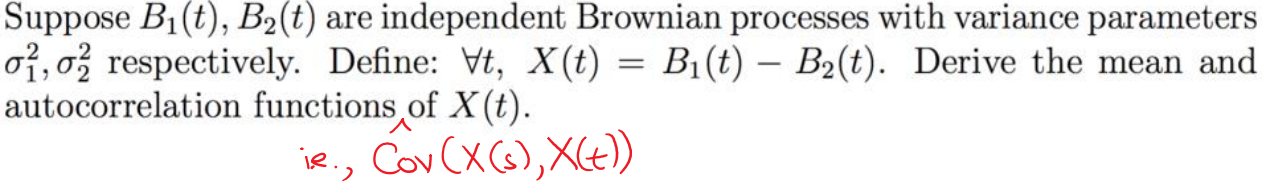
\includegraphics[width=1\linewidth]{image/1.png}
    \end{figure}
    \item 
\end{itemize}

\section{}
\begin{itemize}
    \begin{figure} [H]
        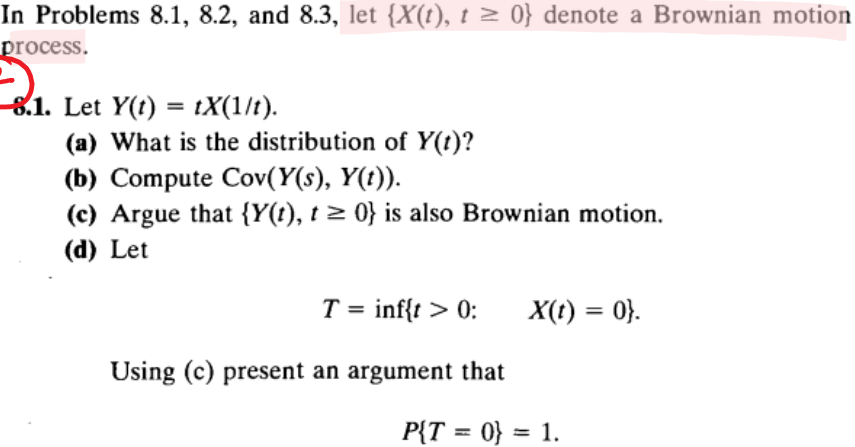
\includegraphics[width=1\linewidth]{image/2.png}
    \end{figure}
    \item 
\end{itemize}

\section{}
\begin{itemize}
    \begin{figure} [H]
        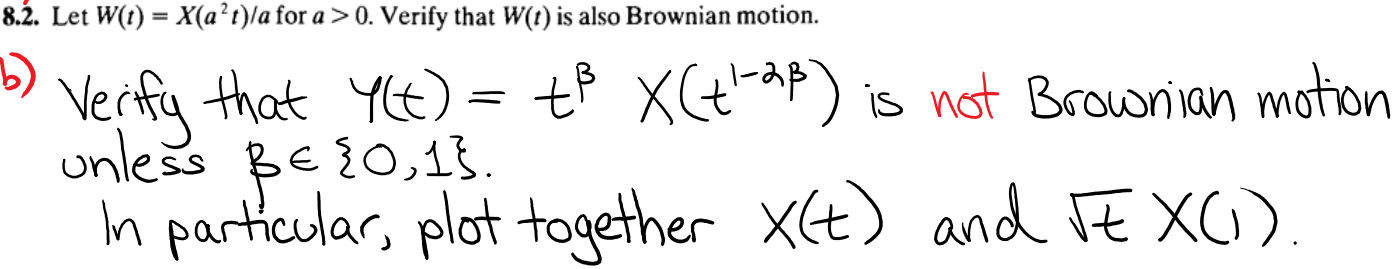
\includegraphics[width=1\linewidth]{image/3.png}
    \end{figure}
    \item 
\end{itemize}

\section{}
\begin{itemize}
    \begin{figure} [H]
        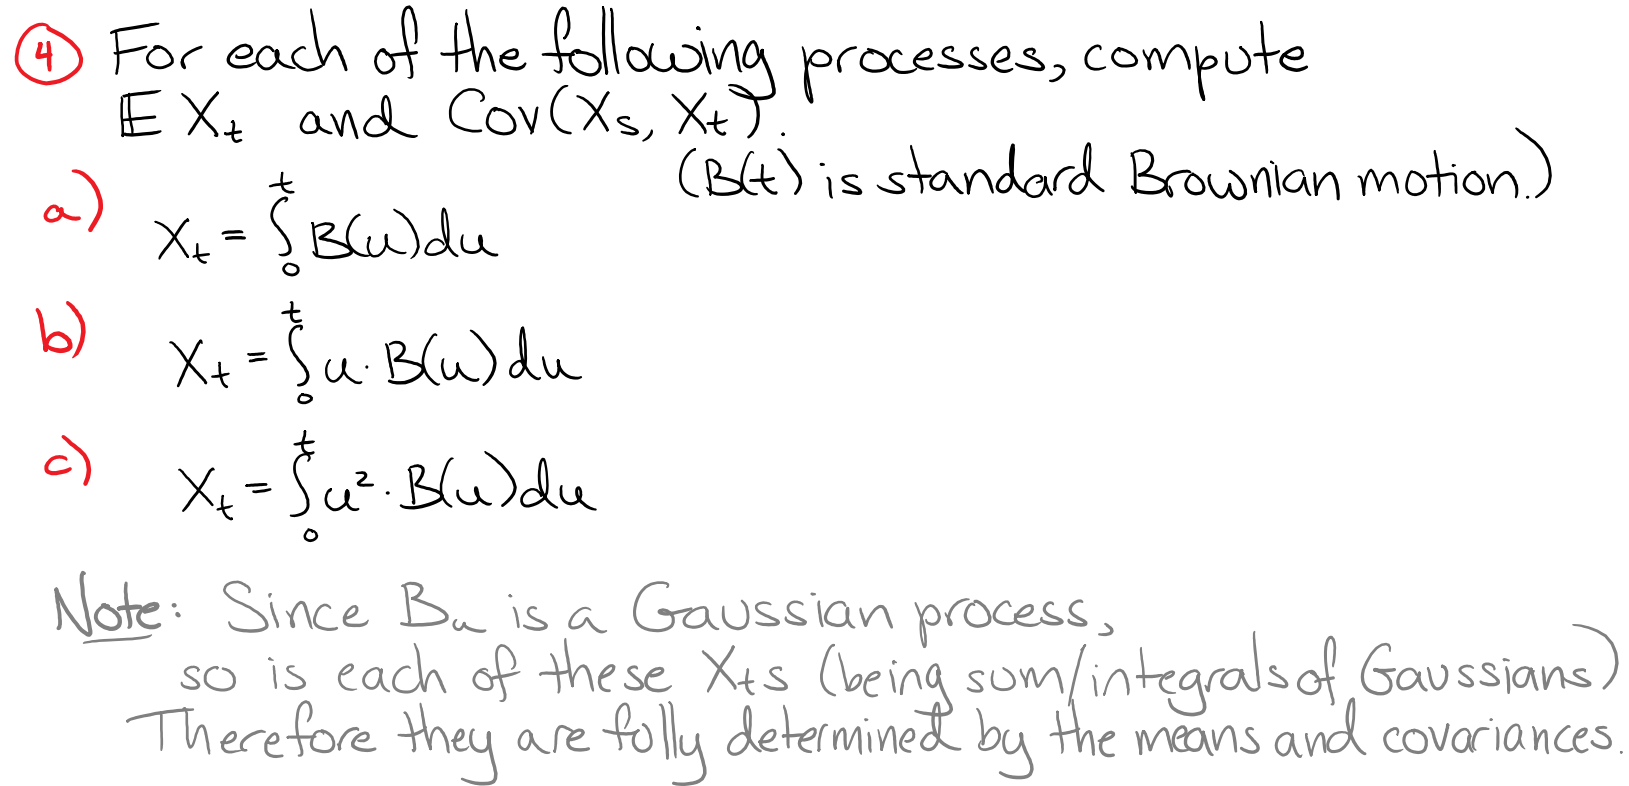
\includegraphics[width=1\linewidth]{image/4.png}
    \end{figure}
    \item 
\end{itemize}

\end{document}
